\chapter{Design}
\addcontentsline{toc}{chapter}{Design}

\section{Software Functionality and Architecture}
	The programme resulting from this work is called ``Tagger3D'', for it's purpose is to tag an RGBD image of an object with a category label. The Bag of Words classification pipeline consists of four main parts discussed previously. In order to determine the best combination of algorithms for any given task an extensive research and evaluation has to be performed. In order to simplify the process the software system should be configurable, extensible and easy to maintain. Moreover, if it is to be used in any realistic setting it has to be efficient as well.
	
	\subsection{Required functionality}	
	There are three major functions that have to be supplied by the programme: (1) estimation, (2) batch inference and (3) inference. The first one is responsible for the model training. In order to perform this operation the following steps have to be completed: (i) detection and description of keypoints on the training set, (ii) codebook generation, (ii) classifier model training. The functions (2) and (3) are somewhat similar. Both require: (i) detection and description of keypoints on the test set, (ii) parsing keypoints' description into a visual vocabulary description and (iii) classification. The only is in the (i) step, e.g. the batch inference requires every image from the test set to be processed, whereas the inference can be done on any single image. The (3) have to be distinguished because it is the function that is to be used in a fully functional system mounted on i.e. a mobile robot.
	
		\subsubsection{Input/Output operations}	
		Additional functionality have to be provided in the field of input/output operations. Before any processing can be done each image have to be read into memory. Both batch inference and estimation are dataset dependant. What I mean by this is that a previously compiled database have to be accessible. The inference, on the other hand, is meant to be used in a production environment i.e. with a Kinect connected only. While the OpenNI Grabber framework from the PointCloud Library is essentially what is required for the inference, a little more elaboration has to be done on the demands of the estimation and batch inference environments. The two third party datasets used in the project have different formats and need to be tackled separately. The B3DO object dataset contains multiple objects in a single image. The locations of the images are available in xml files, while rgb and depth data are stored in separate files, 8-bit 3 channel jpeg and 16 bit one channel png respectively. Single objects have to be extracted from both pictures using the provided annotations and point cloud have to be build. The Zhang's dataset contain single objects. The rgb data is stored in 8 bit 3 channel jpegs and csv files contains euclidean coordinates of every rgb pixel. Both databases contain objects' labels that have to be loaded separately.
		
		A different problem is serialisation. If the models from the training stage are to be used during inference, they have to be serialised. This means that a standardised way of saving and loading of kMeans and SVM models have to be provided.  
	
		\subsubsection{Configuration}		
		Every algorithm employed in the project have several configuration parameters. If the parameters were to be compiled with the code, every change would require a rebuild of the application or its parts. In order to address this issue a means of configuration from outside the code should be provided. 
		
		\subsubsection{Interchangeability of algorithms}		
		Multitude of available algorithms makes it time consuming and computationally expensive to evaluate every available option. It should be possible to compile the programme with many algorithms suitable for performing the same task and decide which one should be used at run-time.
		
	\subsection{Architecture}
	
	\begin{figure}[ht]
	\centering
	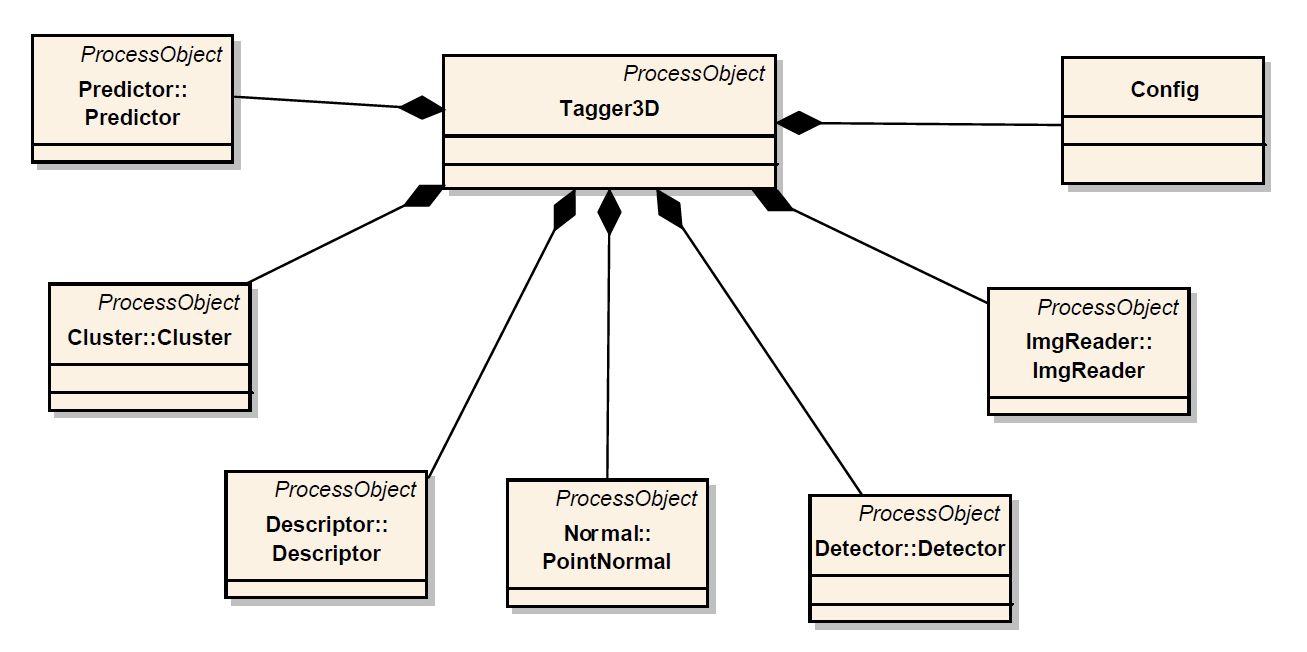
\includegraphics[width=1.0\textwidth]{figs/short}
	\caption{Tagger3D class diagram}
	\label{fig:class_diagram}
	\end{figure}
	
	The described functionality can be achieved in the following way. The utilisation of Object Oriented Programming (OOP) can lead to production of modular, flexible and extensible software. Using C++ as the language of choice can result in high efficiency. The excellent meta-programming tools provided by the C++ language help minimise the length of resulting hand-written code.
	
	\subsubsection{Configurability}
	In order to achieve configurability all the configuration parameters are stored in a configuration file. A separate object has been constructed for configuration file parsing. Simply called `Config', it makes use of the Boost.program\_options library to parse both the configuration file and command line arguments. It returns an associative array of (parameter, value) pairs. The convention is that if an object has to be configured the configuration map has to be passed in the object's constructor (other constructors are private).
	
	\subsubsection{Strategy Design Pattern}
	
	\begin{figure}[ht]
	\centering
	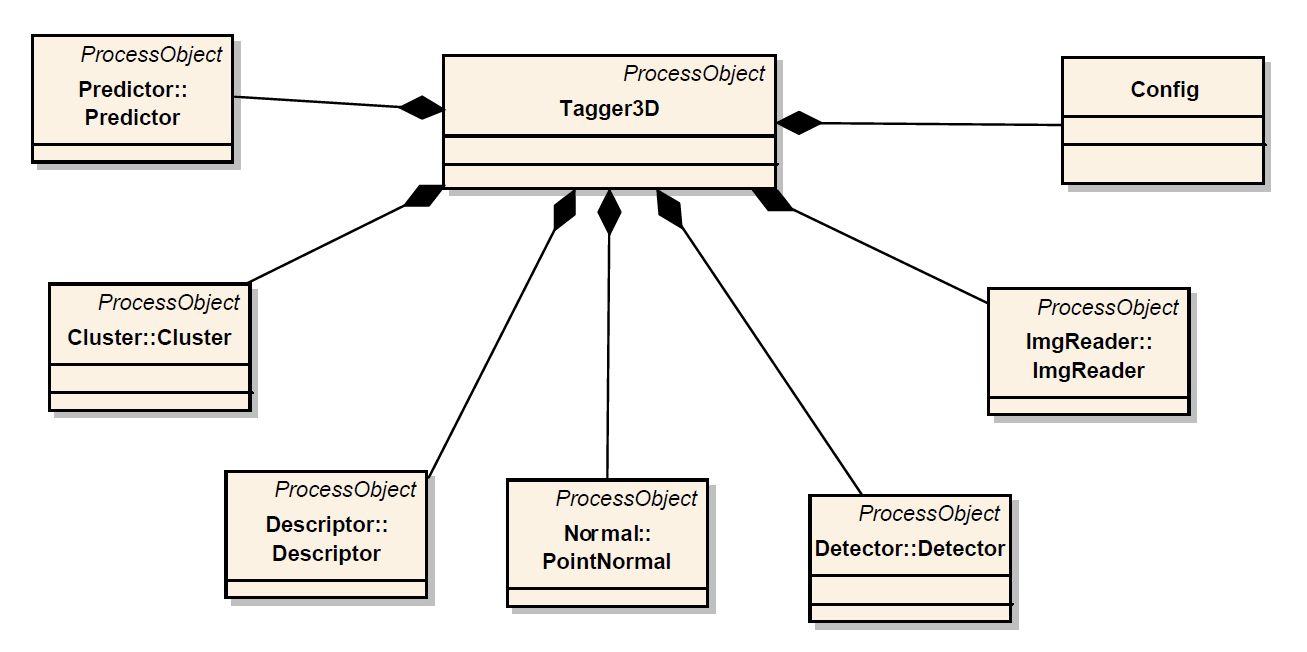
\includegraphics[width=1.0\textwidth]{figs/short}
	\caption{Strategy pattern}
	\label{fig:strategy}
	\end{figure}
	
	Design patterns has been introduced for the very first time by Gamma \emph{et al} in \cite{gamma1993design}. They are best practices that should be used to solved common, recurring problems in software design. One of the patterns is the strategy pattern. It enables implementation of multiple algorithms handling some task and selection the desired behaviour at run-time. It is the exact problem encountered here. It is stated that an interface should be defined for each task and multiple classes encapsulating different algorithms for handling the tasks should realise those interfaces. One modification has been done: Algorithms have often some common operations, thus an idea of an interface (a class without any implemented methods) was dropped in favour of a virtual class. 
	
	The strategy pattern was used for every processing step of the pipeline so as to make it extensible. One might want to enhance this solution by using an abstract factory design pattern, which has not been done in this case. It might make the code easier to maintain and read. However, the project is relatively small and the bulk of an abstract factory is unnecessary.
	
	There six five classes that can be treated as algorithms' interfaces in a strategy pattern. They are: ImgReader, PointNormal, Detector, Descriptor, Cluster, Predictor. Each of them contains pure virtual computation methods --- 'read` in case of the ImgReader or 'predict' in case of the Predictor. Additionally, they have some common methods defined --- I/O methods in Cluster or batch processing methods (such that take a vector of elements instead of a single element as input) for the Detector and the Descriptor. Every pure virtual class has its specialisations. For example there is the PFHDescriptor class with a Point Feature Histogram descriptor or a KMeansCluster employing kMeans clustering algorithm. The Tagger3D class chooses specialisations of the algorithms at run-time, depending on the configuration parameters.
	
	